\section{Establishing the Eigenfunction Property}
\label{Ch4:Sec:Eig}

% Prove that the 2 eigenfunctions are, indeed, Fourier eigenfunctions!

In this section, we show that the $\pm$-Eigenfunctions are, indeed, $\pm$-Eigenfunctions of the Fourier transform.

In the previous section, we did not work with $a$ and $b$ directly as it was sufficient to work with $a\rad$ and $b\rad$ instead. In this section, however, we will need to use the following formula for the $n$-dimensional Fourier transform of the $n$-dimensional Gaussian.

\begin{boxtheorem}[Fourier Transform of a Gaussian]\label{Ch4:Thm:GaussianFourier}
    Fix $n \in \N$ and $b \in \C$, with $\Re(b) > 0$. If $F : \R^n \to \C$ is given by
    \begin{align*}
        F(x) = e^{-b \norm{x}^2}
    \end{align*}
    then for all $\xi \in \R^n$, the Fourier transform of $F$ is given by
    \begin{align*}
        \hat{F}\of{\xi} = \parenth{\frac{\pi}{b}}^{{n} / {2}} e^{{- \pi^2 \norm{\xi}^2} / {b}}
    \end{align*}
\end{boxtheorem}
A \href{https://github.com/leanprover-community/mathlib4/blob/5a2eaa85c555c4263e15928cef249cbaad2eb2d2/Mathlib/Analysis/SpecialFunctions/Gaussian/FourierTransform.lean#L360-L363}{formal proof} exists in \mathlib.

We will also need the following version of the \CGT, which allows us to deform contours of integration in the complex plane.

\begin{boxtheorem}[Cauchy-Goursat: Squares and Circles]\label{Ch4:Thm:CGTRectCircle}
    Fix $w \in \C$ and $r > 0$. Let $\gamma$ be the quarter-circle parametrised by $\gamma(t) = w + r\pcos{t} + \abs{r} i \psin{t}$ for $0 \leq t \leq \pi/2$. For any $f : \C \to \C$ that is holomorphic in the region enclosed by $\gamma$ and the line segments from $w + r$ to $w + r + ir$ and $w + r + ir$ to $w + ir$, we have
    \begin{align*}
        \int_{\gamma} f(z) \, \diff{z}
        = \int_{w + r}^{w + r + ir} f(z) \, \diff{z} + \int_{w + r + ir}^{w + ir} f(z) \, \diff{z}
    \end{align*}
\end{boxtheorem}

While this is an immediate consequence of the more general (and well-known) \CGT\ from complex analysis, there are numerous challenges involved in formalising this and other versions of the theorem. We will discuss it in \Cref{Ch5:Sec:Cauchy-Goursat}. We also note that the above result implies an analogous result that can be proved by a change of variables. See \Cref{Ch4:Subfig:CGTRectCircle_Alt}.

\begin{figure}[ht]
    \centering
    \begin{subfigure}{0.48\linewidth}
        \centering
        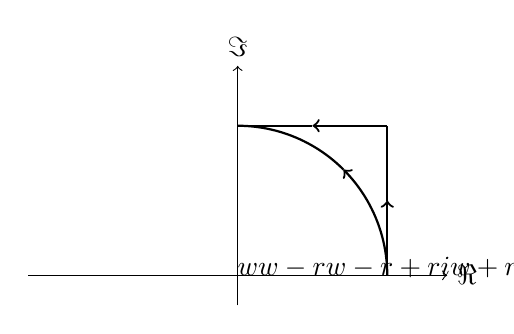
\begin{tikzpicture}[scale=1.9]
            % Axes
            \draw[->] (-1.4,0) -- (1.4,0) node[right] {$\Re$};
            \draw[->] (0,-0.2) -- (0,1.4) node[above] {$\Im$};
        
            % Quarter-circle contour
            \draw[thick, domain=0:45, ->] plot ({cos(\x)}, {sin(\x)});
            \draw[thick, domain=45:90, -] plot ({cos(\x)}, {sin(\x)});

            % Rectangular contour
            \draw[thick, ->] (1,0) -- (1,0.5);
            \draw[thick, -] (1,0.5) -- (1,1);
            \draw[thick, ->] (1,1) -- (0.5,1);
            \draw[thick, -] (0.5,1) -- (0,1);

            % Points of interest
            \labelledpoint{0}{0}{-0.3}{-0.8}{$w$}
            \labelledpoint{1}{0}{0}{-0.8}{$w - r$}
            \labelledpoint{1}{1}{0.3}{-0.2}{$w - r + ri$}
            \labelledpoint{0}{1}{-0.7}{-0.5}{$w + ri$}
        \end{tikzpicture}
        \caption{Contours for which \Cref{Ch4:Thm:CGTRectCircle} holds.}
    \end{subfigure} 
    \hfill
    \begin{subfigure}{0.48\linewidth}
        \centering
        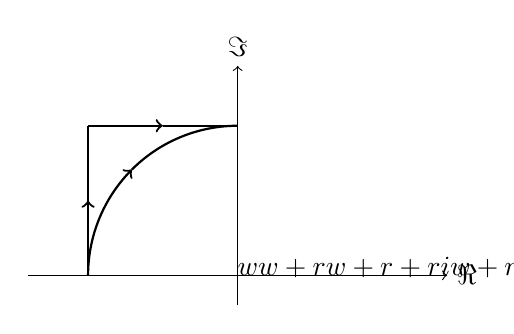
\begin{tikzpicture}[scale=1.9]
            % Axes
            \draw[->] (-1.4,0) -- (1.4,0) node[right] {$\Re$};
            \draw[->] (0,-0.2) -- (0,1.4) node[above] {$\Im$};
        
            % Quarter-circle contour
            \draw[thick, domain=180:135, ->] plot ({cos(\x)}, {sin(\x)});
            \draw[thick, domain=135:90, -] plot ({cos(\x)}, {sin(\x)});

            % Rectangular contour
            \draw[thick, ->] (-1,0) -- (-1,0.5);
            \draw[thick, -] (-1,0.5) -- (-1,1);
            \draw[thick, ->] (-1,1) -- (-0.5,1);
            \draw[thick, -] (-0.5,1) -- (0,1);

            % Points of interest
            \labelledpoint{0}{0}{0.3}{-0.8}{$w$}
            \labelledpoint{-1}{0}{0}{-0.8}{$w + r$}
            \labelledpoint{-1}{1}{-0.3}{-0.2}{$w + r + ri$}
            \labelledpoint{0}{1}{0.7}{-0.5}{$w + ri$}
        \end{tikzpicture}
        \caption{Contours for which an analogous result holds.}
        \label{Ch4:Subfig:CGTRectCircle_Alt}
    \end{subfigure} 
    \caption{The contour deformations permitted by \Cref{Ch4:Thm:CGTRectCircle}.}
\end{figure}

We now prove that $a$ is indeed a $+1$-eigenfunction of the Fourier transform.

\subsection{The $+1$-Eigenfunction}

The Fourier transform acts very interestingly on $a$. Recall from \Cref{Ch3:Thm:FourierSchwartz_CLE} that the Fourier transform is a linear isomorphism of Schwartz spaces. Since $I_1, \ldots, I_6$ are Schwartz, so are their compositions with the norm-squared function. Hence, for all $x \in \R^8$,
\begin{align*}
    \F\of{a(x)}
    % = \F\of{I_1\of{\norm{x}^2}} + \F\of{I_2\of{\norm{x}^2}} + \F\of{I_3\of{\norm{x}^2}} + \F\of{I_4\of{\norm{x}^2}} + \F\of{I_5\of{\norm{x}^2}} + \F\of{I_6\of{\norm{x}^2}}
    = \F\of{\sum_{j=1}^{6} I_j\of{\norm{x}^2}}
    = \sum_{j=1}^{6} \F\of{I_j\of{\norm{x}^2}}
\end{align*}

The strategy to show that $\F\of{a} = a$ will be to show that $\F$ acts on the $I_j\of{\norm{x}^2}$ in the following manner:\footnote{Note that we are abusing notation by denoting the function $x \mapsto I_j\of{\norm{x}^2} \in \Sch\of{\R^8, \C}$ by $I_j\of{\norm{x}^2}$.}
\begin{align}
    \F\of{I_1\of{\norm{x}^2} + I_2\of{\norm{x}^2}} &= I_3\of{\norm{x}^2} + I_4\of{\norm{x}^2} \label{Ch4:Eq:a_is_eig_perm_12_34} \\
    \F\of{I_3\of{\norm{x}^2} + I_4\of{\norm{x}^2}} &= I_1\of{\norm{x}^2} + I_2\of{\norm{x}^2} \label{Ch4:Eq:a_is_eig_perm_34_12} \\
    \F\of{I_5\of{\norm{x}^2}} &= I_6\of{\norm{x}^2} \label{Ch4:Eq:a_is_eig_perm_5_6} \\
    \F\of{I_6\of{\norm{x}^2}} &= I_5\of{\norm{x}^2} \label{Ch4:Eq:a_is_eig_perm_6_5}
\end{align}
Since, in addition to being Schwartz, all the $I_j\of{\norm{x}^2}$ (and their sums) are radial, \Cref{Ch3:Prop:RadialSchwartzFourier} tells us that \eqref{Ch4:Eq:a_is_eig_perm_34_12} and \eqref{Ch4:Eq:a_is_eig_perm_6_5} follow from \eqref{Ch4:Eq:a_is_eig_perm_12_34} and \eqref{Ch4:Eq:a_is_eig_perm_5_6} respectively. We now prove \eqref{Ch4:Eq:a_is_eig_perm_12_34} and \eqref{Ch4:Eq:a_is_eig_perm_5_6}.

As a preliminary step, though, we need to show integrability.

\begin{boxproposition}\label{Ch4:Prop:FourierIntegralConvergence_Ij}
    Fix $1 \leq j \leq 6$, and write $I_j(r) = \int_{X_j} f(r, z) \, \diff{z}$. Then, the Fourier Integral
    \begin{align*}
        \F\of{I_j\of{\norm{x}^2}}\of{\xi} = \int_{\R^8} \int_{X_j} \abs{f\of{\norm{x}^2, z} \, e^{-2 \pi i \cycl{x, \xi}}} \, \diff{z} \, \diff{x}
    \end{align*}
    converges for all $\xi \in \R^8$.
\end{boxproposition}
\begin{proof}
    Fix $\xi \in \R^8$. Note that we can disregard the $e^{-2 \pi i \cycl{x, \xi}}$ factor since it has absolute value $1$: the only reason we mention it is to emphasise that we are proving that the Fourier integral converges absolutely. Effectively, we need to show that the function
    \begin{align*}
        (x, z) \mapsto f\of{\norm{x}^2, z}
    \end{align*}
    admits an absolutely convergent integral over $\R^8 \times X_j$ with respect to the product measure.
    
    It has been formally verified that \href{https://github.com/leanprover-community/mathlib4/blob/5a2eaa85c555c4263e15928cef249cbaad2eb2d2/Mathlib/MeasureTheory/Integral/Prod.lean#L222-L238}{proving this is equivalent to proving the following two facts}.

    \begin{enumerate}
        \item \textbf{The integral over $X_j$ of the function $z \mapsto f\of{\norm{x}^2, z}$ is absolutely convergent for almost every $x \in \R^8$.}
        
        This is actually true for all $x$, and follows from the arguments in \Cref{Ch4:Subec:Schwartzness_a}.
        
        \item \textbf{The integral over $\R^8$ of the function $x 
        \mapsto \int_{X_j} \abs{f\of{\norm{x^2}, z}} \diff{z}$ is absolutely convergent.}
        
        By inspection, the arguments in \Cref{Ch4:Subec:Schwartzness_a} bound the function $r \mapsto \int_{X_j} \abs{f\of{r, z}} \diff{z}$ by a Schwartz function. Composing with the norm squared preserves Schwartzness by \Cref{Ch3:Prop:Multidimensional_Schwartz_of_Schwartz}, so we can bound the function $x \mapsto \int_{X_j} \abs{f\of{\norm{x}^2, z}} \diff{z}$ by a Schwartz function. It has been formally verified that \href{https://github.com/leanprover-community/mathlib4/blob/5a2eaa85c555c4263e15928cef249cbaad2eb2d2/Mathlib/Analysis/Distribution/SchwartzSpace.lean#L1095-L1097}{Schwartz functions are integrable}, so the integral over $\R^8$ of the function $x \mapsto \int_{X_j} \abs{f\of{\norm{x}^2, z}} \diff{z}$ must be absolutely convergent.
    \end{enumerate}
We can therefore conclude that the Fourier integral converges absolutely.
\end{proof}

Note that the above proposition is stronger than showing merely that the $I_j\of{\norm{x}^2}$ are integrable, as that does not imply that the integrands of the $I_j\of{\norm{x}^2}$ are integrable with respect to the product measure on $\R^8 \times X_j$. \Cref{Ch4:Prop:FourierIntegralConvergence_Ij}, however, does imply this, and we will need this to swap integrals using Fubini's theorem to prove the eigenfunction property.

\begin{boxlemma}\label{Ch4:Lemma:Fourier_I_1_add_I_2_eq_I_3_add_I_4}
    The Fourier transform % $\F : \Sch\of{\R^8, \C} \to \Sch{\R^8, \C}$
    maps $I_1\of{\norm{x}^2} + I_2\of{\norm{x}^2}$ to $I_3\of{\norm{x}^2} + I_4\of{\norm{x}^2}$.
\end{boxlemma}
\begin{proof}
    Since $\F$ acts linearly, we can treat $I_1$ and $I_2$ separately. For the purpose of this proof, denote the Fourier transforms of $I_1\of{\norm{x}^2}$ and $I_2\of{\norm{x}^2}$ by $F_1$ and $F_2$ respectively. Fix $\xi \in \R^8$. The integrability condition in \Cref{Ch4:Prop:FourierIntegralConvergence_Ij} allows us to change the order of integration below:
    \begin{align*}
        F_1\of{\xi} &= \int_{\R^8} \parenth {\int_{-1}^{-1 + i} \phi_0\of{\frac{-1}{z+1}} \, \parenth{z + 1}^2 \, e^{\pi i \norm{x}^2 z} \, \diff{z}} e^{-2\pi i \cycl{x, \xi}} \, \diff{x} \\
        &= \int_{-1}^{-1 + i} \phi_0\of{\frac{-1}{z+1}} \, \parenth{z + 1}^2 \parenth{\int_{\R^8} e^{\pi i \norm{x}^2 z} e^{-2\pi i \cycl{x, \xi} \diff{x}}} \, \diff{z}
    \end{align*}
    We can express $F_2$ in an analogous fashion. In both cases, the inner integral is exactly the Fourier integral of a Gaussian: in the notation of \Cref{Ch4:Thm:GaussianFourier}, $b = \pi i z$, and since $\Im(z) = \Re\of{i z} > 0$, we may apply the theorem to conclude that the inner integral is just
    \begin{align*}
        \frac{1}{z^4} \, e^{-\pi i \norm{\xi}^2 / z}
    \end{align*}
    We may therefore write
    \begin{align*}
        F_1\of{\xi} &= \int_{-1}^{-1 + i} \phi_0\of{\frac{-1}{z+1}} \, \parenth{z + 1}^2z^{-4} \, e^{\pi i \norm{\xi}^2 \parenth{\frac{-1}{z}}} \, \diff{z} \\
        F_2\of{\xi} &= \int_{-1 + i}^{i} \phi_0\of{\frac{-1}{z+1}} \, \parenth{z + 1}^2z^{-4} \, e^{\pi i \norm{\xi}^2 \parenth{\frac{-1}{z}}} \, \diff{z}
    \end{align*}
    We make a change of variables $w = \frac{-1}{z}$ in the above integrals. This Möbius transformation turns the vertical and horizontal contours in $F_1$ and $F_2$ into quarter-circular contours that we denote $\gamma_1$ and $\gamma_2$ respectively. See \Cref{Ch4:Fig:Eigenfunction_Mobius_Contours}.

    \begin{figure}[htb]
        \centering
        \begin{subfigure}{0.4\linewidth}
            \centering
            \begin{tikzpicture}[scale=1.9]
                % Axes
                \draw[->] (-1.4,0) -- (1.4,0) node[right] {$\Re$};
                \draw[->] (0,-0.2) -- (0,1.4) node[above] {$\Im$};
    
                % F_1
                \draw[thick, ->] (-1,0) -- (-1,0.5);
                \draw[thick, -] (-1,0.5) -- (-1,1);

                % F_2
                \draw[thick, ->] (-1,1) -- (-0.5,1);
                \draw[thick, -] (-0.5,1) -- (0,1);
    
                % Points of interest
                % \labelledpoint{0}{0}{0.3}{-0.8}{$0$}
                \labelledpoint{-1}{0}{0}{-0.8}{$-1$}
                \labelledpoint{-1}{1}{-0.3}{-0.2}{$-1 + i$}
                \labelledpoint{0}{1}{0.3}{-0.4}{$i$}
            \end{tikzpicture}
            \caption{Before the transformation}
        \end{subfigure}
        \begin{subfigure}{0.1\linewidth}
            \vfill
            \[ \leadsto \]
            \vspace{5em}
        \end{subfigure}
        \begin{subfigure}{0.4\linewidth}
            \centering
            \begin{tikzpicture}[scale=1.9]
                % Axes
                \draw[->] (-1.4,0) -- (1.4,0) node[right] {$\Re$};
                \draw[->] (0,-0.2) -- (0,1.4) node[above] {$\Im$};
            
                % \gamma_1
                \draw[thick, domain=0:45, ->] plot ({0.5 + 0.5 * cos(\x)}, {0.5 * sin(\x)}) node[below left] {$\gamma_1$};
                \draw[thick, domain=45:90, -] plot ({0.5 + 0.5 * cos(\x)}, {0.5 * sin(\x)});

                % \gamma_2
                \draw[thick, domain=0:45, ->] plot ({0.5 * cos(\x)}, {0.5 + 0.5 * sin(\x)}) node[below left] {$\gamma_2$};
                \draw[thick, domain=45:90, -] plot ({0.5 * cos(\x)}, {0.5 + 0.5 * sin(\x)});
    
                % Points of interest
                % \labelledpoint{0}{0}{0.3}{-0.8}{$w$}
                \labelledpoint{1}{0}{0}{-0.8}{$1$}
                \labelledpoint{0.5}{0.5}{0.6}{-0.2}{$\frac{1}{2} + \frac{1}{2}i$}
                \labelledpoint{0}{1}{-0.3}{-0.4}{$i$}
            \end{tikzpicture}
            \caption{After the transformation}
        \end{subfigure}
        \caption{The effect of the Möbius transformation $z \mapsto -1/z$ on the contours of $F_1$ and $F_2$}
        \label{Ch4:Fig:Eigenfunction_Mobius_Contours}
    \end{figure}
    Treating $\xi$ as a constant and denoting
    \begin{align*}
        f(w) := \phi_0\of{-1 - \frac{1}{w - 1}} \, \parenth{\frac{-1}{w} + 1}^2 w^2 \, e^{\pi i \norm{\xi}^2 w}
    \end{align*}
    we can distribute the $w^2$ term and use the fact that $\phi_0$ is $1$-periodic (cf. \eqref{Ch4:Eq:phi_0_add_one}) to write
    \begin{align*}
        f(w) = \phi_0\of{\frac{-1}{w - 1}} \, \parenth{w - 1}^2 \, e^{\pi i \norm{\xi}^2 w}
    \end{align*}
    we note that $f$ is holomorphic (in $w$) on the upper half-plane. \Cref{Ch4:Thm:CGTRectCircle} then tells us that
    \begin{align*}
        F_1\of{\xi}
        &= \int_{\gamma_1} f(w) \, \diff{w}
        = \int_{1}^{1 + \frac{1}{2}i} f(w) \, \diff{w}
        + \int_{1 + \frac{i}{2}i}^{\frac{1}{2} + \frac{1}{2}i} f(w) \, \diff{w} \\
        F_2\of{\xi}
        &= \int_{\gamma_2} f(w) \, \diff{w}
        = \int_{\frac{1}{2} + \frac{1}{2}i}^{\frac{1}{2} + i} f(w) \, \diff{w}
        + \int_{\frac{1}{2} + i}^{i} f(w) \, \diff{w}
    \end{align*}
    The \CGT\ for rectangles, which has been \href{https://github.com/leanprover-community/mathlib4/blob/88928cefd7edb1ba61623bffd4e86389dfe1f648/Mathlib/Analysis/Complex/CauchyIntegral.lean#L245}{formally verified}, tells us that
    \begin{align*}
        \int_{1 + \frac{i}{2}i}^{\frac{1}{2} + \frac{1}{2}i} f(w) \, \diff{w}
        + \int_{\frac{1}{2} + \frac{1}{2}i}^{\frac{1}{2} + i} f(w) \, \diff{w}
        = \int_{1 + \frac{1}{2}i}^{1+i} f(w) \, \diff{w}
        + \int_{1+i}^{\frac{1}{2} + i} f(w) \, \diff{w}
    \end{align*}
    Therefore, we can express $F_1 + F_2$ in the following manner:
    \begin{align*}
        F_1\of{\xi} + F_2\of{\xi}
        &= \int_{1}^{1 + \frac{1}{2}i} f(w) \, \diff{w}
        + \parenth{\int_{1 + \frac{i}{2}i}^{\frac{1}{2} + \frac{1}{2}i} f(w) \, \diff{w}
        + \int_{\frac{1}{2} + \frac{1}{2}i}^{\frac{1}{2} + i} f(w) \, \diff{w}}
        + \int_{\frac{1}{2} + i}^{i} f(w) \, \diff{w} \\
        &= \parenth{\int_{1}^{1 + \frac{1}{2}i} f(w) \, \diff{w}
        + \int_{1 + \frac{1}{2}i}^{1+i} f(w) \, \diff{w}}
        + \parenth{\int_{1+i}^{\frac{1}{2} + i} f(w) \, \diff{w}
        + \int_{\frac{1}{2} + i}^{i} f(w) \, \diff{w}} \\
        &= I_3\of{\norm{\xi}^2} + I_4\of{\norm{\xi}^2}
    \end{align*}
    as required. \Cref{Ch4:Fig:Eigenfunction_CauchyGoursat_a} shows how contours were modified over the course of this argument.
    \begin{figure}[hbt]
        \centering
        \begin{subfigure}{0.4\linewidth}
            \centering
            \begin{tikzpicture}[scale=1.9]
                % Axes
                \draw[->] (-1.4,0) -- (1.4,0) node[right] {$\Re$};
                \draw[->] (0,-0.2) -- (0,1.4) node[above] {$\Im$};
            
                % \gamma_1
                \draw[thick, domain=0:45, ->, red] plot ({0.5 + 0.5 * cos(\x)}, {0.5 * sin(\x)}) node[below left] {$\gamma_1$};
                \draw[thick, domain=45:90, -, red] plot ({0.5 + 0.5 * cos(\x)}, {0.5 * sin(\x)});

                % \gamma_2
                \draw[thick, domain=0:45, ->, red] plot ({0.5 * cos(\x)}, {0.5 + 0.5 * sin(\x)}) node[below left] {$\gamma_2$};
                \draw[thick, domain=45:90, -, red] plot ({0.5 * cos(\x)}, {0.5 + 0.5 * sin(\x)});

                % Rectangle 1
                \draw[thick, ->, darkgreen] (1, 0) -- (1, 0.25);
                \draw[thick, -, darkgreen] (1, 0.25) -- (1, 0.5);
                \draw[thick, ->, darkgreen] (1, 0.5) -- (0.75, 0.5);
                \draw[thick, -, darkgreen] (0.75, 0.5) -- (0.5, 0.5);

                % Rectangle 2
                \draw[thick, ->, darkgreen] (0.5, 0.5) -- (0.5, 0.75);
                \draw[thick, -, darkgreen] (0.5, 0.75) -- (0.5, 1);
                \draw[thick, ->, darkgreen] (0.5, 1) -- (0.25, 1);
                \draw[thick, -, darkgreen] (0.25, 1) -- (0, 1);
    
                % Points of interest
                % \labelledpoint{0}{0}{0.3}{-0.8}{$w$}
                \labelledpoint{1}{0}{0}{-0.8}{$1$}
                \labelledpoint{0.5}{0.5}{0.6}{-0.2}{}
                \labelledpoint{0}{1}{-0.3}{-0.4}{$i$}
                \labelledpoint{1}{0.5}{0}{0}{}
                \labelledpoint{0.5}{1}{0}{0}{}
            \end{tikzpicture}
            \caption{Changing contours from circles to rectangles}
        \end{subfigure}
        \hfill
        \begin{subfigure}{0.4\linewidth}
            \centering
            \begin{tikzpicture}[scale=1.9]
                % Axes
                \draw[->] (-1.4,0) -- (1.4,0) node[right] {$\Re$};
                \draw[->] (0,-0.2) -- (0,1.4) node[above] {$\Im$};
            
                % Rectangle 1
                \draw[thick, ->] (1, 0) -- (1, 0.25);
                \draw[thick, -] (1, 0.25) -- (1, 0.5);
                \draw[thick, ->, red] (1, 0.5) -- (0.75, 0.5);
                \draw[thick, -, red] (0.75, 0.5) -- (0.5, 0.5);

                % Rectangle 2
                \draw[thick, ->, red] (0.5, 0.5) -- (0.5, 0.75);
                \draw[thick, -, red] (0.5, 0.75) -- (0.5, 1);
                \draw[thick, ->] (0.5, 1) -- (0.25, 1);
                \draw[thick, -] (0.25, 1) -- (0, 1);

                % Rectangle Cauchy-Goursat
                \draw[thick, ->, darkgreen] (1, 0.5) -- (1, 0.75);
                \draw[thick, -, darkgreen] (1, 0.5) -- (1, 1);
                \draw[thick, ->, darkgreen] (1, 1) -- (0.75, 1);
                \draw[thick, -, darkgreen] (0.75, 1) -- (0.5, 1);
    
                % Points of interest
                % \labelledpoint{0}{0}{0.3}{-0.8}{$w$}
                \labelledpoint{1}{0}{0}{-0.8}{$1$}
                \labelledpoint{0.5}{0.5}{0.6}{-0.2}{}
                \labelledpoint{0}{1}{-0.3}{-0.4}{$i$}
                \labelledpoint{1}{0.5}{0}{0}{}
                \labelledpoint{0.5}{1}{0}{0}{}
                \labelledpoint{1}{1}{0}{0}{}
            \end{tikzpicture}
            \caption{Changing rectangular contours to get $I_3$ and $I_4$}
        \end{subfigure}
        \caption{Applying the two versions of the \CGT\ to prove the result. In the proof, contours were changed from red to green.}
        \label{Ch4:Fig:Eigenfunction_CauchyGoursat_a}
    \end{figure}
\end{proof}

The proof that the Fourier transform maps $I_5$ to $I_6$ is nearly identical in structure but significantly simpler, because the Möbius transformation $z \mapsto \frac{-1}{z}$ simply maps the contour in $I_5$ to that in $I_6$ (and vice-versa). We omit the proof.

In summary, we have shown that the Fourier transform permutes the integrals that make up $a$, thereby not changing $a$. $a$ is thus an eigenfunction of $\F$ with eigenvalue $1$.

It is worth noting that the Möbius transformation $z \mapsto \frac{-1}{z}$ in the proof of \Cref{Ch4:Lemma:Fourier_I_1_add_I_2_eq_I_3_add_I_4} has derivative $\frac{1}{z^2}$, which reduces the $z^4$ term in the integrand to $z^2$, which matches the pattern in $I_3$ and $I_4$. However, the reason the $z^4$ term arises is that we take the $8$-dimensional Fourier transform of an $8$-dimensional Gaussian. This illustrates why it was necessary to treat $a$ as an $\R^8 \to \C$ function to show the eigenfunction property. More generally, despite Fourier transforms being linear isomorphisms of Schwartz spaces, the fact remains that in different Schwartz spaces, the Fourier transform operators may be fundamentally different, and linear maps between Schwartz spaces are not guaranteed to preserve the Fourier transform operator.

We now use similar techniques to show that $b$ is a Fourier eigenfunction with eigenvalue $-1$. % Just as we did with the proof of Schwartzness, we omit repetitive arguments and focus on the key distinctions between the two cases.

\subsection{The $-1$-Eigenfunction}

Just as with the integrals of $a$, the $8$-dimensional Fourier transform permutes the integrals that make up $b$. The difference, however, is that it reverses signs in the process. Specifically,
\begin{align}
    \F\of{J_1\of{\norm{x}^2} + J_2\of{\norm{x}^2}} &= -J_3\of{\norm{x}^2} - J_4\of{\norm{x}^2} \label{Ch4:Eq:b_is_eig_perm_12_34} \\
    \F\of{I_5\of{\norm{x}^2}} &= -I_6\of{\norm{x}^2} \label{Ch4:Eq:b_is_eig_perm_5_6}
\end{align}
with the inverse results following from linearity and \Cref{Ch3:Prop:RadialSchwartzFourier}.

First, we note that in the integrability proof of the $I_j$ (\Cref{Ch4:Prop:FourierIntegralConvergence_Ij}), we did not use any properties of the $I_j$ that do not hold for the $J_j$: the same integrability conditions hold for $J_j$ because they were bounded in \Cref{Ch4:Subec:Schwartzness_b} in an analogous manner to the $I_j$ in \Cref{Ch4:Subec:Schwartzness_a}.

We are now ready to prove an analogue of \Cref{Ch4:Lemma:Fourier_I_1_add_I_2_eq_I_3_add_I_4}.

\begin{boxlemma}\label{Ch4:Lemma:Fourier_J_1_add_J_2_eq_neg_J_3_sub_J_4}
    The Fourier transform maps $J_1\of{\norm{x}^2} + J_2\of{\norm{x}^2}$ to $-J_3\of{\norm{x}^2} - J_4\of{\norm{x}^2}$.
\end{boxlemma}
\begin{proof}
    Again, since $\F$ acts linearly, we can treat $J_1$ and $J_2$ separately. For the purpose of this proof, denote the Fourier transforms of $J_1\of{\norm{x}^2}$ and $J_2\of{\norm{x}^2}$ by $F_1$ and $F_2$ respectively. As before, we may exchange the order of the integrals in the Fourier integral and write, for all $\xi \in \R^8$,
    \begin{align*}
        F_1 &= \int_{-1}^{-1 + i} \psi_T(z) \, z^{-4} \, e^{\pi i \norm{\xi}^2 \parenth{\frac{-1}{z}}} \, \diff{z} \\
        F_2 &= \int_{-1 + i}^{i} \psi_T(z) \, z^{-4} \, e^{\pi i \norm{\xi}^2 \parenth{\frac{-1}{z}}} \, \diff{z}
    \end{align*}
    Again, we change variables via the Möbius transformation $w = \frac{-1}{z}$. Denoting by $f$ the integrand (with respect to $w$) of $F_1$ and $F_2$, we have
    \begin{align*}
        f(w) = \psi_T\of{\frac{-1}{w}} \, w^2 \, e^{\pi i \norm{\xi}^2 w}
    \end{align*}
    From \eqref{Ch4:Eq:psi_T_eq_zsq_mul_psi_T_neg_inv}, we can see that
    \begin{align*}
        f(w) = -\psi_T\of{w} \, e^{\pi i \norm{\xi}^2 w}
    \end{align*}
    Noting further that $f$ is holomorphic in $w$ because $\psi_T$ can be expressed as a fraction with holomorphic functions and the (non-vanishing on $\Halfplane$) discriminant form in the denominator (cf. \Cref{Ch4:Prop:psi_as_div_disc}), we can prove the result by deforming contours in exactly the same manner as we did in the proof of \Cref{Ch4:Lemma:Fourier_I_1_add_I_2_eq_I_3_add_I_4}. See \Cref{Ch4:Fig:Eigenfunction_CauchyGoursat_a}.
\end{proof}

An analogous argument shows that $\F\of{J_5\of{\norm{x}^2}} = - J_6\of{\norm{x}^2}$. The key difference is that we use the fact that $\psi_S = \psi_I \mid_{-2} S$ (which is true by definition) instead of the fact that $\psi_T \mid_{-2} S = -\psi_T$ (which is nontrivial).\todo{Replace slash rels with eqn nos} We also note that the sign change in the case of $J_5$ comes not from applying a slash relation but from the fact that the Möbius transformation $z \mapsto \frac{-1}{z}$ reverses the direction of the contours.